\definecolor{qqwuqq}{rgb}{0.,0.39215686274509803,0.}
\definecolor{ududff}{rgb}{0.30196078431372547,0.30196078431372547,1.}
\definecolor{cqcqcq}{rgb}{0.7529411764705882,0.7529411764705882,0.7529411764705882}
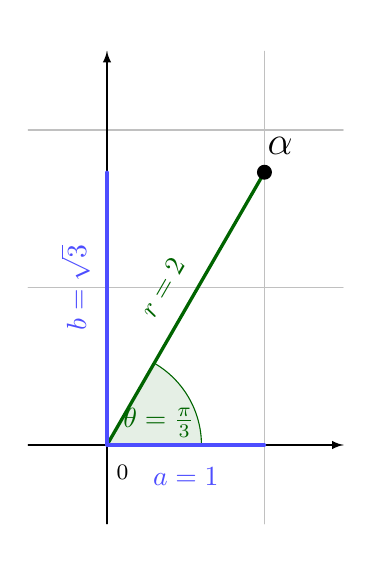
\begin{tikzpicture}[line cap=round,line join=round,>=latex,x=2cm,y=2cm]
\draw [color=cqcqcq,, xstep=2cm,ystep=2cm] (-.5,-.5) grid (1.5,2.5);
\draw[->,color=black] (-.5,0) -- (1.5,0);
\draw[->,color=black] (0.,-.5) -- (0.,2.5);
\draw[color=black] (0pt,-10pt) node[right] {\footnotesize $0$};
\clip(-.5,-.65) rectangle (1.5,2.65);
\draw [shift={(0.,0.)},color=qqwuqq,fill=qqwuqq,fill opacity=0.10000000149011612] (0,0) -- (0.:0.6) arc (0.:60.:0.6) -- cycle;
\draw[color=qqwuqq,very thick] (0.,0.)-- (1.,1.7320508075688772);
\draw[color=ududff,very thick] (0.,0.)-- (0,1.7320508075688772);
\draw[color=ududff,very thick] (0.,0.)-- (1.,0);
\draw [fill=black] (1.,1.7320508075688772) circle (2.5pt);
\draw[color=black] (1.1,1.9) node {\Large $\alpha$};
\draw[color=ududff] (.5,-.2) node {$a=1$};
\draw[color=ududff] (-.2,1) node {\rotatebox{90}{$b =\sqrt{3}$}};
\draw[color=qqwuqq] (0.35,1) node {\rotatebox{60}{$r = 2$}};
\draw[color=qqwuqq] (0.33,0.14) node {$\theta = \frac{\pi}{3}$};
\end{tikzpicture}